% include all necessary latex libraries
\documentclass[aspectratio=169,presentation]{beamer}
\usetheme{Boadilla}
\useinnertheme{default}

% -- locale-setup --------------------------------------------------------------

\usepackage[utf8]{inputenc}
\usepackage[T1]{fontenc}
\usepackage[ngerman]{babel}
\usepackage{lmodern}
\usepackage[locale=DE, mode=math, list-final-separator={ oder },
            range-phrase={ bis }, scientific-notation=false, 
            group-digits=integer] {siunitx}

% -- package-includes ----------------------------------------------------------

\usepackage{tikz}
\usepackage{xcolor}
\usetikzlibrary{positioning,automata,matrix,arrows.meta,fit}
\usepackage{graphicx} % including images
\usepackage[font=small,labelfont=bf]{caption} % captions of tables and figures

% -- listing setup -------------------------------------------------------------

\usepackage{listings}
\definecolor{pblue}{rgb}{0.13,0.13,1}
\definecolor{pgreen}{rgb}{0,0.5,0}
\definecolor{pred}{rgb}{0.9,0,0}
\definecolor{pgrey}{rgb}{0.46,0.45,0.48}
\definecolor{javared}{rgb}{0.6,0,0} % for strings
\definecolor{javagreen}{rgb}{0.25,0.5,0.35} % comments
\definecolor{javapurple}{rgb}{0.5,0,0.35} % keywords
\definecolor{javadocblue}{rgb}{0.25,0.35,0.75} % javadoc

\lstset{language=vhdl,
	basicstyle=\ttfamily,
	keywordstyle=\color{javapurple}\bfseries,
	stringstyle=\color{javared},
	commentstyle=\color{javagreen},
	morecomment=[s][\color{javadocblue}]{/**}{*/},
	tabsize=2,
	showspaces=false,
	showstringspaces=false
}

% -- custom commands -----------------------------------------------------------

% just prints given text in large text and on empty frame.
\newcommand{\sectionframe} [1] {
	\begin{frame}
		\vfill
		\Huge
		\centering
		\usebeamercolor[fg]{title}
		#1
		\vfill
		\par
	\end{frame}
}

% wrapper-command to make pretty title takes
% 1=short-title 2=long-title 3=terminnumber 4=date
\newcommand{\maketitlepage} [5] {
  \title[#1]{#2}
  \subtitle{Termin #3}
  \date{#4}
  \author[Jakob Otto]{Jakob Otto}
  \institute{HAW Hamburg}
  \subject{#1}
  \pgfdeclareimage[height=0.5cm, width=1.3cm]{university-logo}{#5}
  \logo{\href{https://www.haw-hamburg.de}{\pgfuseimage{university-logo}}}
  \begin{frame} {}
    \titlepage
  \end{frame}
}

% draws a link symbol
\newcommand{\externalLink} {
  \tikz[x=1.2ex, y=1.2ex, baseline=-0.05ex]{
    \begin{scope}[x=1ex, y=1ex]
      \clip (-0.1,-0.1) 
        --++ (-0, 1.2) 
        --++ (0.6, 0) 
        --++ (0, -0.6) 
        --++ (0.6, 0) 
        --++ (0, -1);
      \path[draw, 
        line width = 0.5, 
        rounded corners=0.5] 
      (0,0) rectangle (1,1);
    \end{scope}
      \path[draw, line width = 0.5] (0.5, 0.5) 
        -- (1, 1);
    \path[draw, line width = 0.5] (0.6, 1) 
      -- (1, 1) -- (1, 0.6);
  }
}

% Adds a circled number -> Looks better than the default
\newcommand{\circled} [1] {
  \tikz[baseline=(char.base)]{
    \node[shape=circle,draw,inner sep=2pt, text centered, text width = .2cm] (char) {#1};
  }
}

% -- extra includes go here ----------------------------------------------------
\usepackage{tikz}
\usepackage[customcolors]{hf-tikz}
\usetikzlibrary{shapes,arrows, positioning, fit, backgrounds}

\newcommand{\connectlr} [3] {
  \path (#1.east) -- (#1.north east) coordinate[pos=0.5] (tmp11);
  \path (#2.west) -- (#2.north west) coordinate[pos=0.5] (tmp21);
  \draw[-latex] (tmp21) -- (tmp11);
  \path (#1.east) -- (#1.south east) coordinate[pos=0.5] (tmp12);
  \path (#2.west) -- (#2.south west) coordinate[pos=0.5] (tmp22);
  \draw[-latex] (tmp12) -- (tmp22);
  \path (#1) -- (#2) node [midway] {\circled{#3}};
}

\newcommand{\connecttb} [3] {  
  \path (#1.south) -- (#1.south west) coordinate[pos=0.5] (tmp11);
  \path (#2.north) -- (#2.north west) coordinate[pos=0.5] (tmp21);
  \draw[-latex] (tmp21) -- (tmp11);
  \path (#1.south) -- (#1.south east) coordinate[pos=0.5] (tmp12);
  \path (#2.north) -- (#2.north east) coordinate[pos=0.5] (tmp22);
  \draw[-latex] (tmp12) -- (tmp22);
  \path (#1) -- (#2) node [midway] {\circled{#3}};
}

%-------------------------------------------------------------------------------
%	Variablen
%-------------------------------------------------------------------------------

\newcommand{\terminnumber}{9}
\newcommand{\hawlogo}{../presentation-template/figs/logo-haw-2017}
\newcommand{\kratzen}{../presentation-template/figs/kratzen}
\newcommand{\aufgabenzettellink}{https://users.informatik.haw-hamburg.de/~schafers/LOCAL/S19W_CE/Aufgabenzettel_Nr5_v09.pdf}

%-------------------------------------------------------------------------------
%	Dokument
%-------------------------------------------------------------------------------

\begin{document}
  \maketitlepage {CE Tutorium} {Tutorium zu\\Computer-Engineering\\im WS19}
  {\terminnumber} {\today} {\hawlogo}

  %-----------------------------------------------------------------------------
  %	Ablauf
  %-----------------------------------------------------------------------------
  \section{Was steht an?}
  \begin{frame}{Ablauf}
    \begin{columns}
      \column{0.6\textwidth}
        \begin{itemize}
          \item Aufgabenzettel Nr 5
          \item Metastabile Zustände
          \item Asynchrone Kommunikation
          \begin{itemize}
            \item 4 Phasen Handshake
          \end{itemize}
          \item Statemachines in VHDL
          \item VHDL-teil 4-Phasen Handshake
        \end{itemize}
      \column{0.4\textwidth}
        
\includegraphics[width=0.6\textwidth]{\kratzen}
    \end{columns}
  \end{frame}

  %-----------------------------------------------------------------------------
  %	Aufgabenzettel
  %-----------------------------------------------------------------------------

  \section{Aufgabenzettel 5}
  \sectionframe{\link{https://users.informatik.haw-hamburg.de/~schafers/LOCAL/S19S_CE/Aufgabenzettel_Nr5_v08.pdf}{Aufgabenzettel 5}}

  %-----------------------------------------------------------------------------
  %	Metastabile Zustände
  %-----------------------------------------------------------------------------

  \section{Metastabile Zustände}
  \sectionframe{Metastabile Zustände}
  \begin{frame} {Metastabile Zustände}
    \begin{alertblock} {}
      Zustand des Signals ist nicht klar definiert\\
      Irgendwas zwischen '1' und '0'
    \end{alertblock}
    \begin{block} {Was ist das?}
      \begin{itemize}
        \item Signale sind nicht unmittelbar stabil
        \begin{itemize}
          \item Brauchen kurz bis gewünschter Zustand erreicht ist
        \end{itemize}
        \item Set-up hold-time greift hier ($\rightarrow$ DT)
        \item Signal kann also zur \glqq{}falschen\grqq{} Zeit abgetastet werden
        \begin{itemize}
          \item [$\rightarrow$] Metastabile Zustände sind die Folge
        \end{itemize}
      \end{itemize}
    \end{block}
  \end{frame}


  \begin{frame} {Metastabile Zustände}
    \begin{figure}[ht]
      \centering
      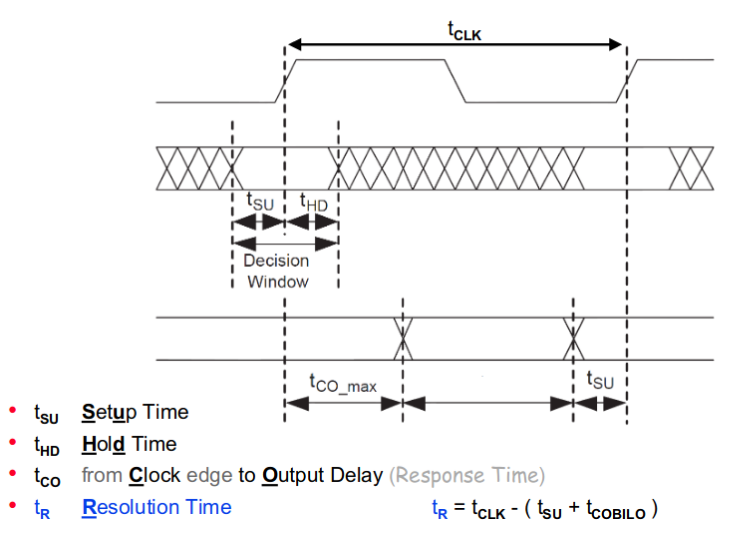
\includegraphics[width=0.7\textwidth]{figs/signalverlauf.png}
      \caption{Darstellung des clk-signals}
    \end{figure}
  \end{frame}

  %-----------------------------------------------------------------------------
  %	Asynchrone Kommunikation
  %-----------------------------------------------------------------------------

  \section{Asynchrone Kommunikation}
  \begin{frame} {Asynchrone Kommunikation}
    \begin{block} {}
      \begin{itemize}
        \item Endpunkte nutzen oft unterschiedlichen Takt
        \item Deshalb Kommunikation zwischen Endpunkten asynchron
        \item Es muss also synchronisiert werden
      \end{itemize}
    \end{block}
    \begin{alertblock} {}
      Kurzschlüsse und Korrupte Daten können entstehen!
    \end{alertblock}
  \end{frame}

  %-----------------------------------------------------------------------------
  %	4 Phasen Handshake
  %-----------------------------------------------------------------------------

  \section{4 Phasen Handshake}
  \begin{frame} {4 Phasen Handshake}
    \begin{block} {}
      \begin{itemize}
        \item Protokoll zum synchronen Übermitteln von Daten
        \item Bidirektional über einen 'x'-bit Datenbus
        \item Verhindert:
        \begin{itemize}
          \item Metastabile Zustände
          \item Kurzschlüsse
        \end{itemize}
      \end{itemize}
    \end{block}
  \end{frame}

  \begin{frame} {4 Phasen Handshake}
    \begin{block} {Welche Leitungen werden benötigt?}
      \begin{itemize}
        \item RD/nWR - signal zum lesen/schreiben signalisieren
        \item REQ - Request vom Master zu Slave
        \item ACK/nRDY - acknowledge vom Slave zum Master
        \item Data - 'x' bit Datenbus
      \end{itemize}
    \end{block}
  \end{frame}

  \subsection{Lesender Zugriff}
  \begin{frame} {Lesender Zugriff}
    \begin{columns}
      \column{0.3\textwidth}
      \column{0.4\textwidth}
        \begin{block} {}
          \begin{enumerate}
            \setcounter{enumi}{0}
            \item Master initiiert RD/nWR = '1'\\
                  Datenbus auf high-impedance\\
                  REQ auf '1'
          \end{enumerate}
        \end{block}
        \begin{block} {}
          \begin{enumerate}
            \setcounter{enumi}{1}
            \item Slave reagiert\\
                  legt geforderte Daten auf Datenbus \\
                  acknowledged (ACK = '1')
          \end{enumerate}
        \end{block}
        \begin{block} {}
          \begin{enumerate}
            \setcounter{enumi}{2}
            \item Master quittiert Empfang\\
                  REQ = '0'
          \end{enumerate}
        \end{block}
        \begin{block} {}
          \begin{enumerate}
            \setcounter{enumi}{3}
            \item Slave nimmt Daten vom Bus\\
            Datenbus auf High-impedance
          \end{enumerate}
        \end{block}
      \column{0.3\textwidth}
    \end{columns}
  \end{frame}


  \begin{frame} {Lesender Zugriff}
    \begin{figure}[ht]
      \centering
      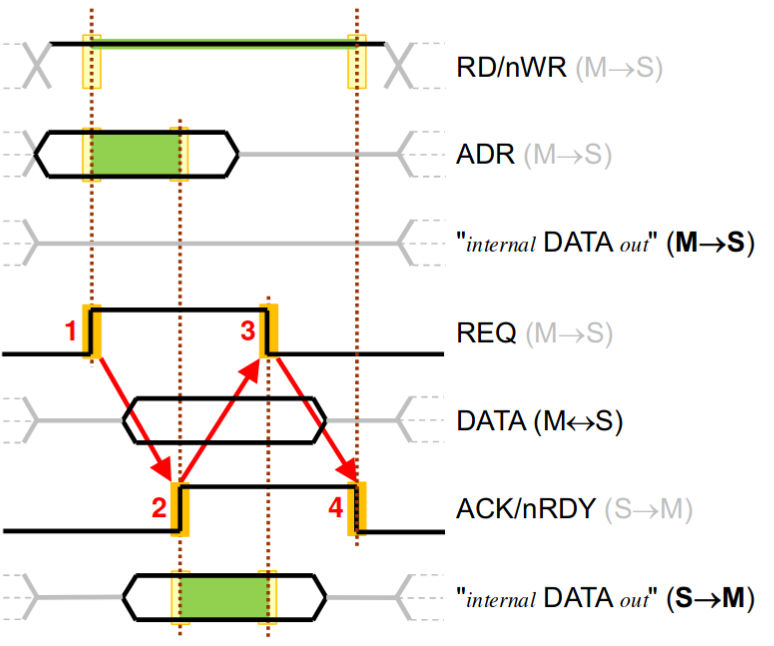
\includegraphics[height=0.7\textheight]{figs/lesen_phase.png}
      \caption{4-Phasen-Handshake lesender Zugriff}
    \end{figure}
  \end{frame}


  \begin{frame} [fragile]
    \begin{lstlisting} [language=C]
  uint16_t  rxdat;
  // wait for the fpga to be ready
  while(READY == 0);

  // setup the connection to the FPGA
  OUTPUT_DISABLE;
  SET_READ;

  // handle transaction by 4 phase handshake
  REQ_ENABLE;
  while(ACKNOWLEDGE == 0);
  rxdat = (GPIOE->IDR & 0x0000FFFF);
  REQ_DISABLE;
  while(ACKNOWLEDGE != 0);

  return rxdat;
    \end{lstlisting}
  \end{frame}

  \subsection{Schreibender Zugriff}
  \begin{frame} {Schreibender Zugriff}
    \begin{columns}
      \column{0.3\textwidth}
      \column{0.4\textwidth}
        \begin{block} {}
          \begin{enumerate}
            \setcounter{enumi}{0}
            \item Master initiiert RD/nWR = '0'\\
                  legt Daten auf Bus \\
                  REQ auf '1'
          \end{enumerate}
        \end{block}
        \begin{block} {}
          \begin{enumerate}
            \setcounter{enumi}{1}
            \item Slave quittiert\\
                  ACK = '1'
          \end{enumerate}
        \end{block}
        \begin{block} {}
          \begin{enumerate}
            \setcounter{enumi}{2}
            \item Master setzt Bus auf High-impedance\\
                  REQ = '0'
          \end{enumerate}
        \end{block}
        \begin{block} {}
          \begin{enumerate}
            \setcounter{enumi}{3}
            \item slave quittiert quittung\\
                  ACK = '0'
          \end{enumerate}
        \end{block}
      \column{0.3\textwidth}
    \end{columns}
  \end{frame}

  \begin{frame} {Schreibender Zugriff}
    \begin{figure}[ht]
      \centering
      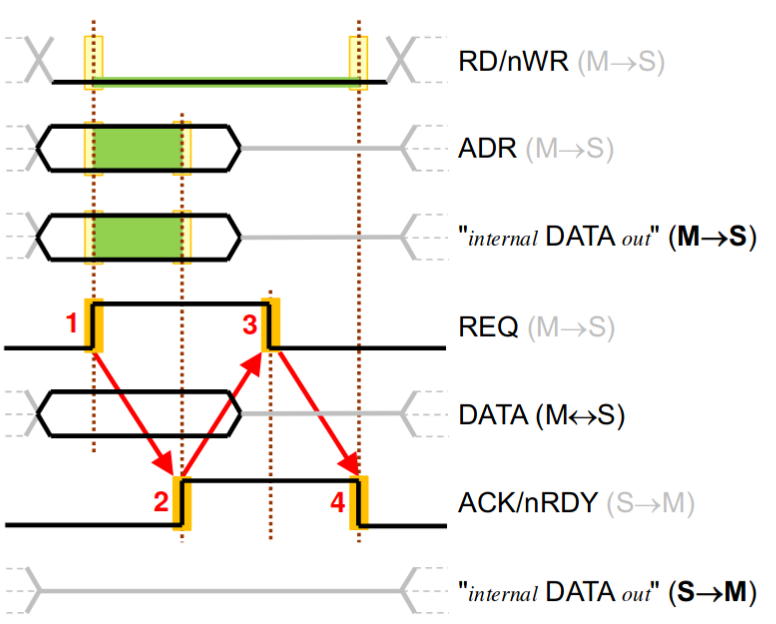
\includegraphics[height=0.7\textheight]{figs/schreibender_zugriff.png}
      \caption{4-Phasen-Handshake lesender Zugriff}
    \end{figure}
  \end{frame}

  \begin{frame} [fragile]
    \begin{lstlisting} [language=C]
  // setup connection to the FPGA
  SET_WRITE;

  OUTPUT_ENABLE;
  // set data
  GPIOE->ODR = txdat;

  // handle transaction by 4 phase handshake
  REQ_ENABLE;
  while(ACKNOWLEDGE == 0);
  REQ_DISABLE;
  while(ACKNOWLEDGE != 0);
    \end{lstlisting}
  \end{frame}

  %-----------------------------------------------------------------------------
  %	FPGA Seite 4 Phasen handshake
  %-----------------------------------------------------------------------------

  \section{Tristate Buffer}
  \begin{frame} [fragile] {Tristate buffer}
    \begin{columns}
      \column{0.5\textwidth}
        Tri-State Treiber für Datenbus
        \begin{lstlisting} [language=vhdl]
  tristate:
  process (oe_s, dato_s) is
  begin
    if oe_s = '1' then
      data <= dato_s;
    else
      data <= (others=>'Z');
    end if;
  end process tristate;
  --
  dati_s <= data;
        \end{lstlisting}
      \column{0.5\textwidth}
        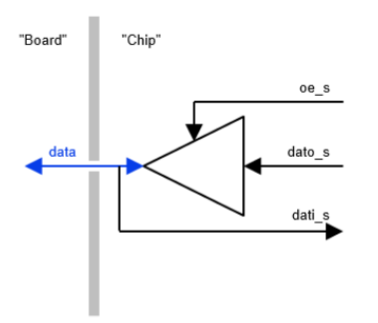
\includegraphics[width=\textwidth]{figs/tristate-treiber.png}
    \end{columns}
  \end{frame}

  \section{4 Phasen handshake in VHDL}
  \begin{frame} {4 Phasen handshake Controller}
    \begin{block} {}
      \begin{itemize}
        \item STM-32 Seite (Master) nun klar
        \begin{itemize}
          \item Wie also nun FPGA Seite (Slave)?
        \end{itemize}
        \item 4 Phasen Handshake gut durch Statemachine darstellbar
        \item 4 Zustände
        \item Lesen/Schreiben nicht großartig unterschiedlich
        \begin{itemize}
          \item Nur unterschiede bei Reaktion auf Request
        \end{itemize}
      \end{itemize}
    \end{block}
  \end{frame}


  \begin{frame} {4 Phasen Statemachine}
    \tikzstyle{format} = [draw, thin, fill=blue!20]
    \tikzstyle{medium} = [ellipse, draw, thin, fill=green!20, minimum height=2.5em]
    \begin{center}
      \begin{figure}
        \begin{tikzpicture}[node distance=3cm, auto,>=latex', thick]
          \node[state,initial]   (A)                {$P_1$};
          \node[state]           (B) [right=of A]   {$P_2$};
          \node[state]           (C) [right=of B]   {$P_3$};
          \node[state]           (D) [right=of C]   {$P_4$};
          \path[->] (A) edge node [above] {$REQ$} (B)
                    (B) edge node [above] {$ACK$} (C)
                    (C) edge node [above] {$\overline{REQ}$} (D)
                    (D) edge [bend right=30] node [above] {$\overline{ACK}$} (A);
        \end{tikzpicture}
      \end{figure}
    \end{center}
  \end{frame}

  \begin{frame} [fragile] {Statemachine Aufbau I}
    \begin{block} {Statemachines}
      \begin{itemize}
        \item Sollten eigentlich noch aus DT bekannt sein
        \item hier trotzdem eine kurze Auffrischung!
      \end{itemize}
    \end{block}

    \begin{lstlisting} [language=vhdl]
  -- 2 bit - 4 states
  signal state_ns : std_logic_vector(1 downto 0);
  signal state_cs : std_logic_vector(1 downto 0) := (others=>'0');
    \end{lstlisting}
  \end{frame}

  \begin{frame} [fragile] {Statemachine Aufbau II}
    \vspace{-.3cm}
    \begin{lstlisting}
  state_v := state_cs;
  case state_cs is
    when "00" =>
      -- state 1
      state_v := "01";
    when "01" =>
      -- state 2
      state_v := "10";
    when "10" =>
      -- state 3
      state_v := "00";
    when others =>
      -- default case
  end case;
  state_ns <= state_v;
    \end{lstlisting}
  \end{frame}

  \sectionframe{Die einzelnen States schaut ihr euch so an :)}

  \begin{frame} {State 1}
    \begin{block} {State 1}
      \begin{itemize}
        \item Read?
        \begin{itemize}
          \item oe $\leftarrow$ 1
          \item dato $\leftarrow$ fx
        \end{itemize}
        \item Write?
        \begin{itemize}
          \item oe $\leftarrow$ 0
          \item req $\leftarrow$ 1
          \item rdy $\leftarrow$ 0
        \end{itemize}
        \item state $\leftarrow$ 1
      \end{itemize}
    \end{block}
  \end{frame}

  \begin{frame} {State 2}
    \begin{block} {State 2}
      \begin{itemize}
        \item ack $\leftarrow$ 1
        \item req = 0?
        \begin{itemize}
          \item oe $\leftarrow$ 0
          \item state $\leftarrow$ 2
        \end{itemize}
      \end{itemize}
    \end{block}
  \end{frame}

  \begin{frame} {State 3}
    \begin{block} {State 3}       
      \begin{itemize}
        \item ack $\leftarrow$ 0
        \item oe $\leftarrow$ 0
        \item state $\leftarrow$ 0
      \end{itemize}
    \end{block}
  \end{frame}

  \begin{frame} {Aufbau Der Schaltung}
    \begin{center}
      \begin{tikzpicture} [    
        auto,
        block/.style={
        rectangle,
        draw=blue,
        thick,
        fill=blue!20,
        text width=5em,
        text centered,
        align=center,
        rounded corners,
        minimum height=2em
        }]
  
        \node[block, text centered,text width = 0.25\textwidth, minimum height=5cm, draw] (stm) {STM32};
      
        \node[block, text width=3cm] (controller) [right=of stm, xshift=5cm, yshift=2cm] {Controller};
        \node[block, text centered,text width = 0.25\textwidth, minimum height = 3 cm, draw] (computer) [below=of controller]{sqrtComputer};
        \node[draw,thick,rounded corners, draw=blue,fit=(controller) (computer)] {};
        
        \path[every node/.style={sloped,anchor=south,auto=false}]
          (stm) edge node [above] {REQ, ACK} node [below] {RD/nWR, DATA} (controller)
  
          (controller) edge [transform canvas={xshift=-1cm}]  node {req} (computer)            
          (controller) edge [transform canvas={xshift=-.3cm}] node {fx} (computer)
          (controller) edge [transform canvas={xshift=.3cm}]  node {x} (computer)
          (controller) edge [transform canvas={xshift=1cm}]  node {rdy} (computer);
  
      \end{tikzpicture}
    \end{center}
  \end{frame}

\end{document}